\documentclass[12pt,letterpaper,hidelinks]{extarticle}
%\usepackage[ansinew]{inputenc}
\usepackage[utf8x]{inputenc}
%\usepackage[latin1]{inputenc}
\usepackage[spanish]{babel}
\usepackage[letterpaper,includeheadfoot, top=1cm, bottom=3.0cm, right=2.0cm, left=2.0cm]{geometry}
\renewcommand{\familydefault}{\sfdefault}

\usepackage{svg}

\usepackage{graphicx}
\usepackage{color}
\usepackage{hyperref}
\usepackage{amssymb}
\usepackage{url}
%\usepackage{pdfpages}
\usepackage{fancyhdr}
\usepackage{hyperref}
\usepackage{subfig}
\usepackage{indentfirst}
\usepackage{titlesec}
\titleformat*{\section}{\large\bfseries}
\titleformat*{\subsection}{\normalsize\bfseries}

\usepackage{listings} %Codigo
\lstset{language=C, tabsize=4,framexleftmargin=5mm,breaklines=true}

\begin{document}
\thispagestyle{empty}
\renewcommand*\listtablename{Índice de tablas}
\renewcommand{\contentsname}{\'Indice}
\renewcommand*{\refname}{}

%\begin{sf}
% --------------- ---------PORTADA --------------------------------------------
\newpage
\pagestyle{fancy}
\fancyhf{}
%-------------------- CABECERA ---------------------
\hbox{
\includegraphics[scale=0.3]{img/fcfm_dcc_png.png} }
%------------------ TÍTULO -----------------------
\vspace*{4cm}
\begin{center}
\Huge  {Tarea 3 - Diccionarios}\\
\vspace{1cm}
\Large {CC4102 - Diseño y Análisis de Algoritmos}\\
\end{center}

%----------------- NOMBRES ------------------------
\vfill
\begin{flushright}
\begin{table}[h]
	\large
  \raggedleft
	\begin{tabular}{ll}
		Alumnos&: Sebastián González\\
				&\ \ Patricio Isbej\\
		Profesor&: Gonzalo Navarro\\
		Auxiliar&: Jorge Bahamonde\\
		Fecha&: \today
	\end{tabular}
\end{table}
\end{flushright}

% ·············· ENCABEZADO - PIE DE PAGINA ············
\newpage
\pagestyle{fancy}
\fancyhf{}

%Encabezado
%\fancyhead[L]{\rightmark}
\fancyhead[L]{\small \rm \textit{Sección \nouppercase\rightmark}} %Izquierda
\fancyhead[R]{\small \rm \textbf{\thepage}} %Derecha


%\fancyfoot[L]{\small \rm \textit{Pie de página - Izquierda}} %Izquierda
%\fancyfoot[R]{\small \rm \textit{Pie de página - Derecha}} %Derecha
%\fancyfoot[C]{\thepage} %Centro

\renewcommand{\sectionmark}[1]{\markright{\thesection.\ #1}}
\renewcommand{\headrulewidth}{0.5pt}
%\renewcommand{\footrulewidth}{0.5pt}

% =============== INDICE ===============
%
%\tableofcontents
%\listoffigures
%\listoftables

% =============== SECCIONES Y SUBSECCIONES ===============
\begin{abstract}
   En este trabajo se analizó 4 estructuras distintas para diccionarios, implementandolas,
	 ejecutandolas para distintos casos y comparando para uno su rendimiento ante inserciones, consultas y eliminaciones.
\end{abstract}
\section{Introducción}
Para este trabajo se compararon los siguientes tipos de diccionarios
	\begin{itemize}
			\item Árbol de Busqueda Binaria convencional
			\item Árbol AVL
		%	\item Splay Tree
	\end{itemize}
	\paragraph{} Árbol de Busqueda Binaria convencional consiste en el árbol donde los elementos son agregados y eliminados a medida que
	se pide, sin realizar ningún tipo de modificación u optimización cuando se hacen las operaciones.
	\paragraph{} Árbol AVL revisa al momento de insertar o eliminar elementos si los hijos de cada nodo involucrado difieren en sus tamaños por
	más de 1, en caso de ocurrir, realiza un rebalanceo de manera que se cumpla la condición
	% \paragraph{} Splay Tree es un árbol en el cual al insertar o consultar por un elemento, este se sube a la raiz del árbol, por medio de
	% rotaciones. También al eliminar un elemento se selecciona su mayor hijo del lado izquierdo o su menor del lado derecho y se sube a la
	% raiz del árbol, usando el mismo método que en la inserción.


 \paragraph{}Para cada estructura se realizaron los siguientes tests

	\begin{itemize}
			\item $2^{4}$ a $2^{14}$ inserciones
			\item $2^{4}$ a $2^{15}$ búsquedas para las estructuras de mayor tamaño
			\item $2^{4}$ a $2^{15}$ borrados
	\end{itemize}

\newpage
\section{Hipótesis}

	\subsection{Árbol de Busqueda Binaria convencional}
		Se espera que para cantidades pequeñas de datos el tiempo de creación de esta estructura
		sea rápida, al no realizar rebalanceos ni cambios extras al realizar operaciones.

		A medida que aumente la cantidad de elementos, se espera que el tiempo de búsqueda e inserción
		tenga forma logarítmica.

	\subsection{Árbol AVL}
		Como este árbol realiza re-balanceos, se espera que el tiempo de creación tome más tiempo que el
		convencional.

		Se espera que para una mayor cantidad de elementos, se comporte mejor que el anterior para todas las operaciones, al encontrarse más comprimido
		 debido a los re-balanceos realizados (va a tener menor altura que el anterior, lo que significa un mejor peor caso).



%	\subsection{Splay Tree}

\section{Diseño e implementación}

\newpage
\section{Experimentos y resultados}

	\begin{figure}[ht!]
		\centering 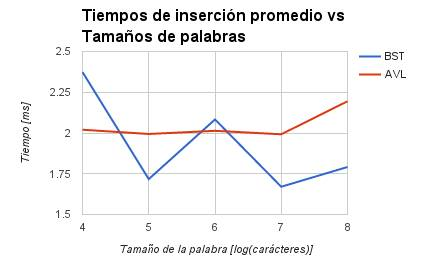
\includegraphics[scale=0.8]{img/ins-size.jpg}
	\end{figure}

	\begin{figure}[ht!]
		\centering 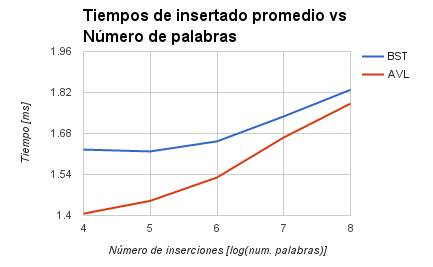
\includegraphics[scale=0.8]{img/ins-num.jpg}
	\end{figure}

\newpage

	\begin{figure}[ht!]
		\centering 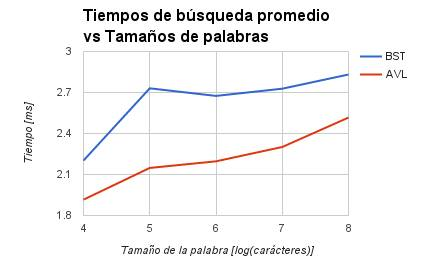
\includegraphics[scale=0.8]{img/srch-size.jpg}
	\end{figure}

	\begin{figure}[ht!]
		\centering 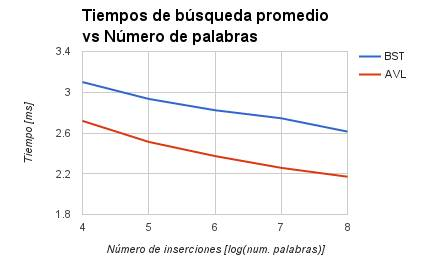
\includegraphics[scale=0.8]{img/srch-num.jpg}
	\end{figure}

\newpage

	\begin{figure}[ht!]
		\centering 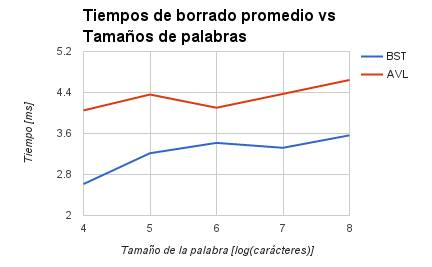
\includegraphics[scale=0.8]{img/del-size.jpg}
	\end{figure}

	\begin{figure}[ht!]
		\centering 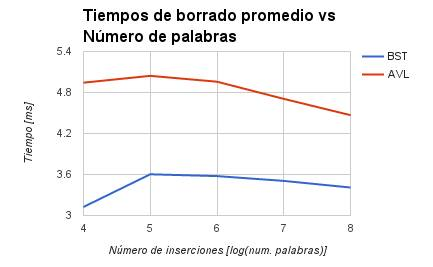
\includegraphics[scale=0.8]{img/del-num.jpg}
	\end{figure}

\newpage
\section{Análisis y Conclusiones}


%%==================== IMAGENES =====================
%% ················ IMAGEN DOBLE ·················
%\begin{figure}[ht!] \centering
%\subfloat[Logo UChile]{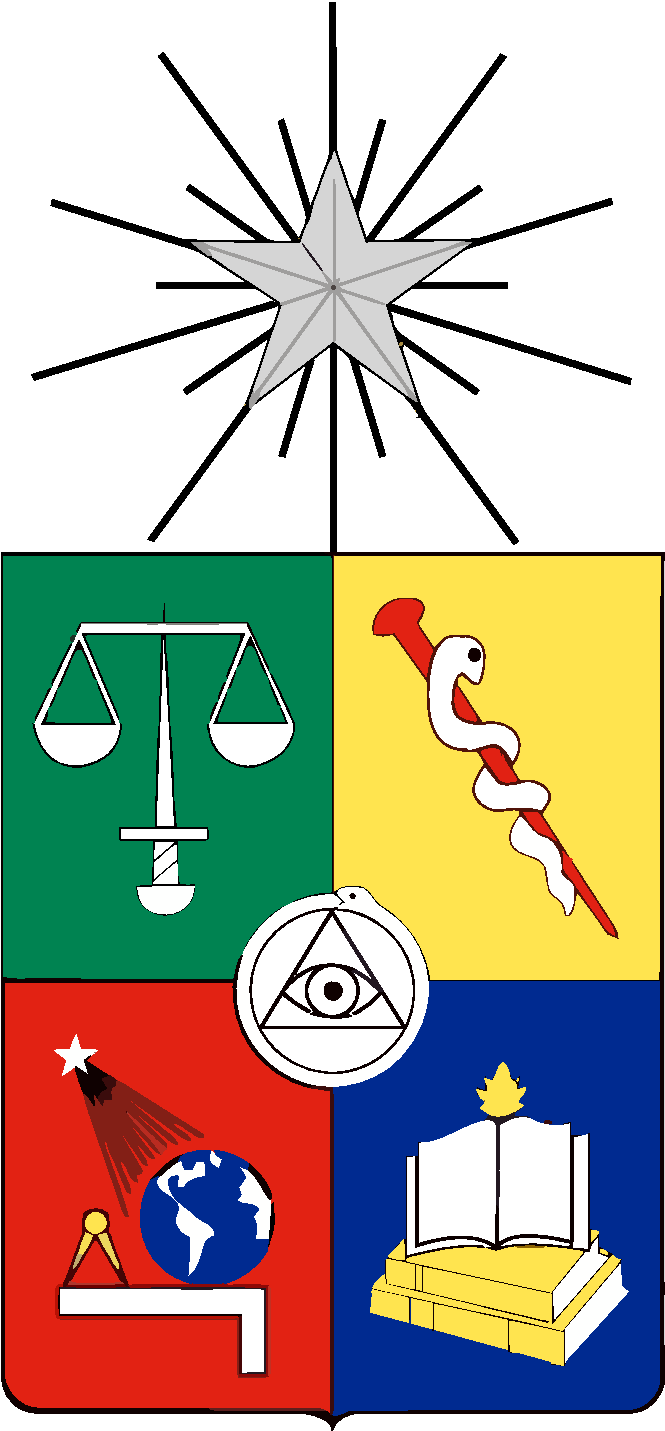
\includegraphics[scale=0.2]{img/escudoU.pdf}}
%\hspace{1cm} %Espacio horizontal
%\subfloat[Logo FCFM]{
\includegraphics[scale=0.45]{img/fcfm.png}}
%\caption{Ejemplo de imagen doble}\label{img1}
%\end{figure}
%%··········································
%
%
%A continuación la figura \ref{img2} presenta otra forma de agregar imágenes
%
%% ················ IMAGENES SIMPLES·················
%\begin{figure}[ht!]
%\centering 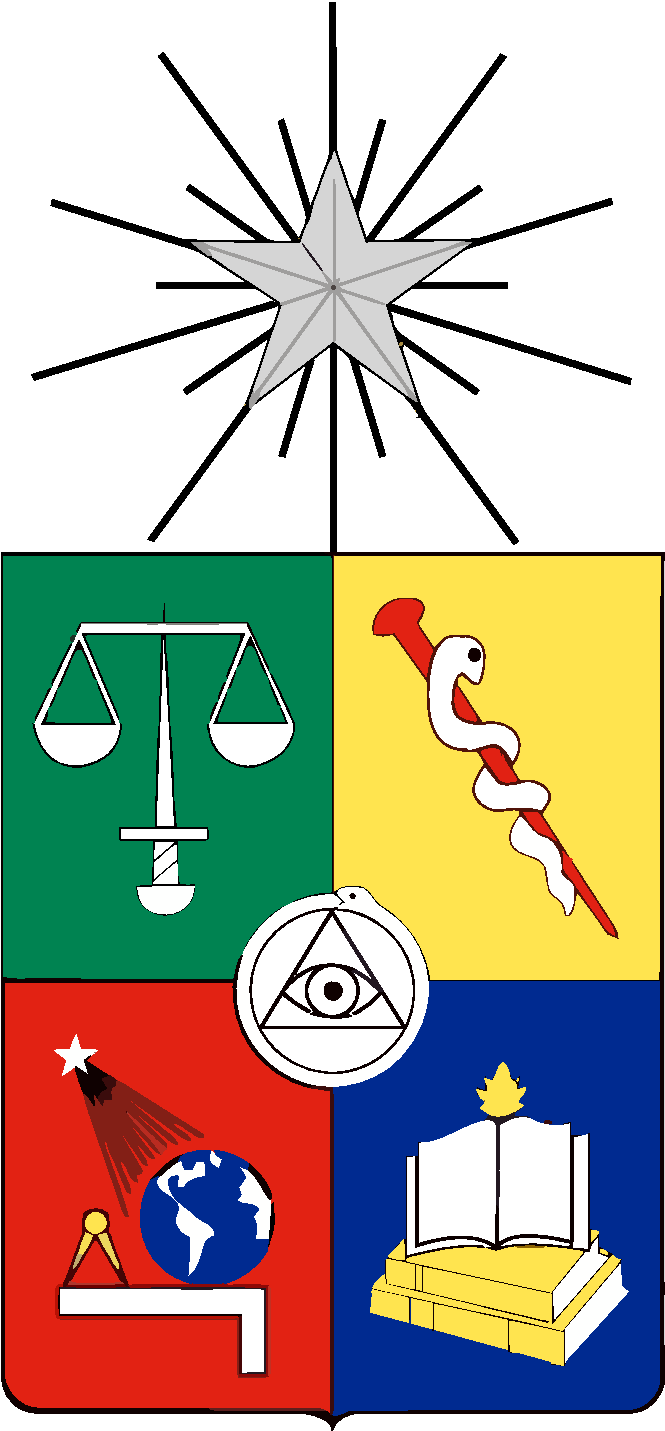
\includegraphics[scale=0.2]{img/escudoU.pdf}
%\caption{Escudo de la Universidad de Chile} \label{img2}
%\end{figure}

%%--------------------------
%
%\begin{figure}[ht!]
%\centering
%\captionsetup{justification=centering,margin=2cm}
%\includegraphics[scale=0.2]{img/fotos_alma/bunkers.JPG}
%\caption{Burros salvajes junto a los bunkers del campamento donde aloja el personal de OSF}
%\label{campamento}
%\end{figure}

%\begin{figure}[ht!]
%\centering \includegraphics[scale=0.2]{img/fotos_alma/cancha_casino.JPG}
%\caption{Multicancha y casino de OSF}
%\label{cancha}
%\end{figure}

%----------------------------
%\begin{figure}[ht!]
%\centering
%\hspace*{-2cm}
%\captionsetup{justification=centering,margin=2cm}
%\includegraphics[scale=0.3]{img/figure_2.pdf}
%\caption{Ejemplo de visualización de un perfil de temperatura usando datos de agosto de 2010}
%\label{surftemp_fig}
%\end{figure}
%\begin{figure}
%\centering
%\hspace*{-2cm}
%\captionsetup{justification=centering,margin=2cm}
%\includegraphics[scale=0.3]{img/figure_3.pdf}
%\caption{Ejemplo de visualización de un perfil de temperatura usando datos de agosto de 2010}
%\label{intliq_fig}
%\end{figure}
%%··········································



%%============== TABLAS ===============
%\begin{table}[h]
% \centering
% \caption{Headers, identificadores y descripción}
% \begin{tabular}{|| c | c | p{7	cm}||}
% \hline
% Identificador de header & Tipo de medición & Descripción \\ [0.5ex]
% \hline\hline
% 10 & - & No se usa (tampoco se describe en el manual)\\
% \hline
% 80 & - & No se usa (tampoco se describe en el manual) \\
% \hline
% 100 & 101 & Tipo de medición y título de los 4 tipos de perfiles\\
% \hline
% 200 & 201 & Header para mediciones meteorológicas a nivel de superficie\\
% \hline
% 300 & 301 & Header para mediciones escalares e integradas\\
% \hline
% 400 & 401, 402, 403, 404 & Ángulo de observación y arreglo de valores de 			altura, la varible independientele (58 valores, de 0 a 10 km), para todos 		los perfiles.\\
% \hline
% \end{tabular}
%\end{table}
%\newpage
%
%Las siguientes cuatro filas contienen el tipo de medición ``101", y especifican el tipo de medición para los cuatro tipos de perfiles.
%
%\begin{table}[h]
% \centering
% \caption{Tipo de perfil y datos}
% \begin{tabular}{||c|c|c|c|c||}
% \hline
% N° de medición & Fecha/Tiempo & 100 &	Tipo de medición & Título \\ [0.5ex]
% \hline\hline
% 1	& 10/07/14 22:07:14 & 101 & 401 & Temperature(K) \\
% \hline
% 2	& 10/07/14 22:07:14 & 101 & 402 & Vapor Density $(g/m^3)$ \\
% \hline
% 3	& 10/07/14 22:07:14 & 101 & 403 & Liquid Density $(g/m^3)$ \\
% \hline
% 4	& 10/07/14 22:07:14 & 101 & 404 & Relative Humidity (\%) \\
% \hline
% \end{tabular}
%\end{table}
%
%El resto de las filas son mediciones (de tipo 201, 301, 401, 402, 403 y 404). \textbf{Estas son las medidas que van a hacer almacenadas en la base de datos}
%\begin{table}[h]
% \centering
% \caption{Ejemplo de mediciones meteorológicas a nivel de superficie y su correspondiente header}
% \begin{tabular}{||c|c|c|c|c|c|c|c||}
% \hline
% Record & Date/Time & 200 & Tamb(K) & Rh(\%) & Pres(mb) & Tir(K) & Rain \\ [0.5ex]
% \hline\hline
% 25 & 10/07/14 22:08:13 & 201 & 276.032 & 10.13 & 557.48 & 191.09 & 0 \\
% \hline
% \end{tabular}
%\end{table}
%
%\newpage
%\begin{table}[h]
% \centering
% \caption{Ejemplo de mediciones de valores scalares e integrados y su correspondiente header}
% \begin{tabular}{||c|c|c|c|c|c|c||}
% \hline
% Record & Date/Time & 300 &	Int. Vapor(cm) & Int. Liquid(mm) & Cloud Base(km) \\ [0.5ex]
% \hline\hline
% 42	& 10/07/14 22:08:56 & 301 & 0.077 & 0 & -1 \\
% \hline
% \end{tabular}
%\end{table}
%
%\begin{table}[h]
% \centering
% \caption{Ejemplo de perfiles y sus correspondientes headers}
% \begin{tabular}{||c|c|c|c|c|c|c||}
% \hline
% Record & Date/Time & 400 &	LV2 Processor(angle) & 0 & ... & 10 \\ [0.5ex]
% \hline\hline
% 46 & 10/07/14 22:09:41 & 401 &	Zenith & 276.017 & ... & 259.11 \\
% \hline
% 53	& 10/07/14 22:09:43 & 402 &	Angle Scan(N) &	0.623 & ... & 0.007 \\
% \hline
% 57	& 10/07/14 22:09:43 & 403 &	Angle Scan(S) &	0.021 & ... & 0.005 \\
% \hline
% 61	& 10/07/14 22:09:43 & 404 &	Angle Scan(A) &	2.805 & ... & 0.336 \\
% \hline
% \end{tabular}
%\end{table}


% ============= REFERENCIAS ==============
%\newpage
%
%\section{Referencias}
%\begin{thebibliography}{99}
%	\bibitem{nodoPag} R. Jacob Baker, \textit{CMOS. Circuit Design, Layout, and Simulation}, 2nd ed., USA: IEEE Press, 2005
%	\bibitem{Bojan} asdasdas
%
%\end{thebibliography}


% ============= FIN DE DOCUMENTO ==============
\end{document}
